\renewcommand{\chaptername}{Capitulo}
\chapter{Metodolog\'ia} 
\label{Metodologia}

El cap\'titulo \ref{Metodologia} se organiza como sigue: al inicio, se determina el modelo o modelos empleados para el desarrollo del servicio web. Despu\'es, se describe el \textit{an\'alisis de requerimientos} determinando las actividades a desarrollar. Posteriormente, en la etapa de \textit{diseño} de desarrollan los modelos de referencia. En la etapa de \textit{implementación}, se desglosan las diferentes etapas el desarrollo del servicio. Finalmente, se establece la herramienta de \textit{evaluaci\'on} y las tareas de \textit{mantenimiento}.

\section{Modelo de desarrollo}

Para el desarrollo del servicio web se emplearon dos dos modelos de desarrollo de software en distintos momentos. Como modelo base, se emplea el de cascada \cite{IngDeSW} para las etapas de an\'alisis de requerimientos y diseño, para las etapas subsecuentes, se adapt\'o el modelo incremental como una etapa m\'as que consiste en la codificación de módulos reducidos, pruebas rápidas de funcionamiento, retroalimentación y corrección, liberación o escalamiento, para terminar con la implementaci\'on del servicio web con una etapa final de mantenimiento como se muestra en la Figura \ref{modeloDesarrolloSW}

\begin{figure}[!ht]
	\centering
	\fbox{
	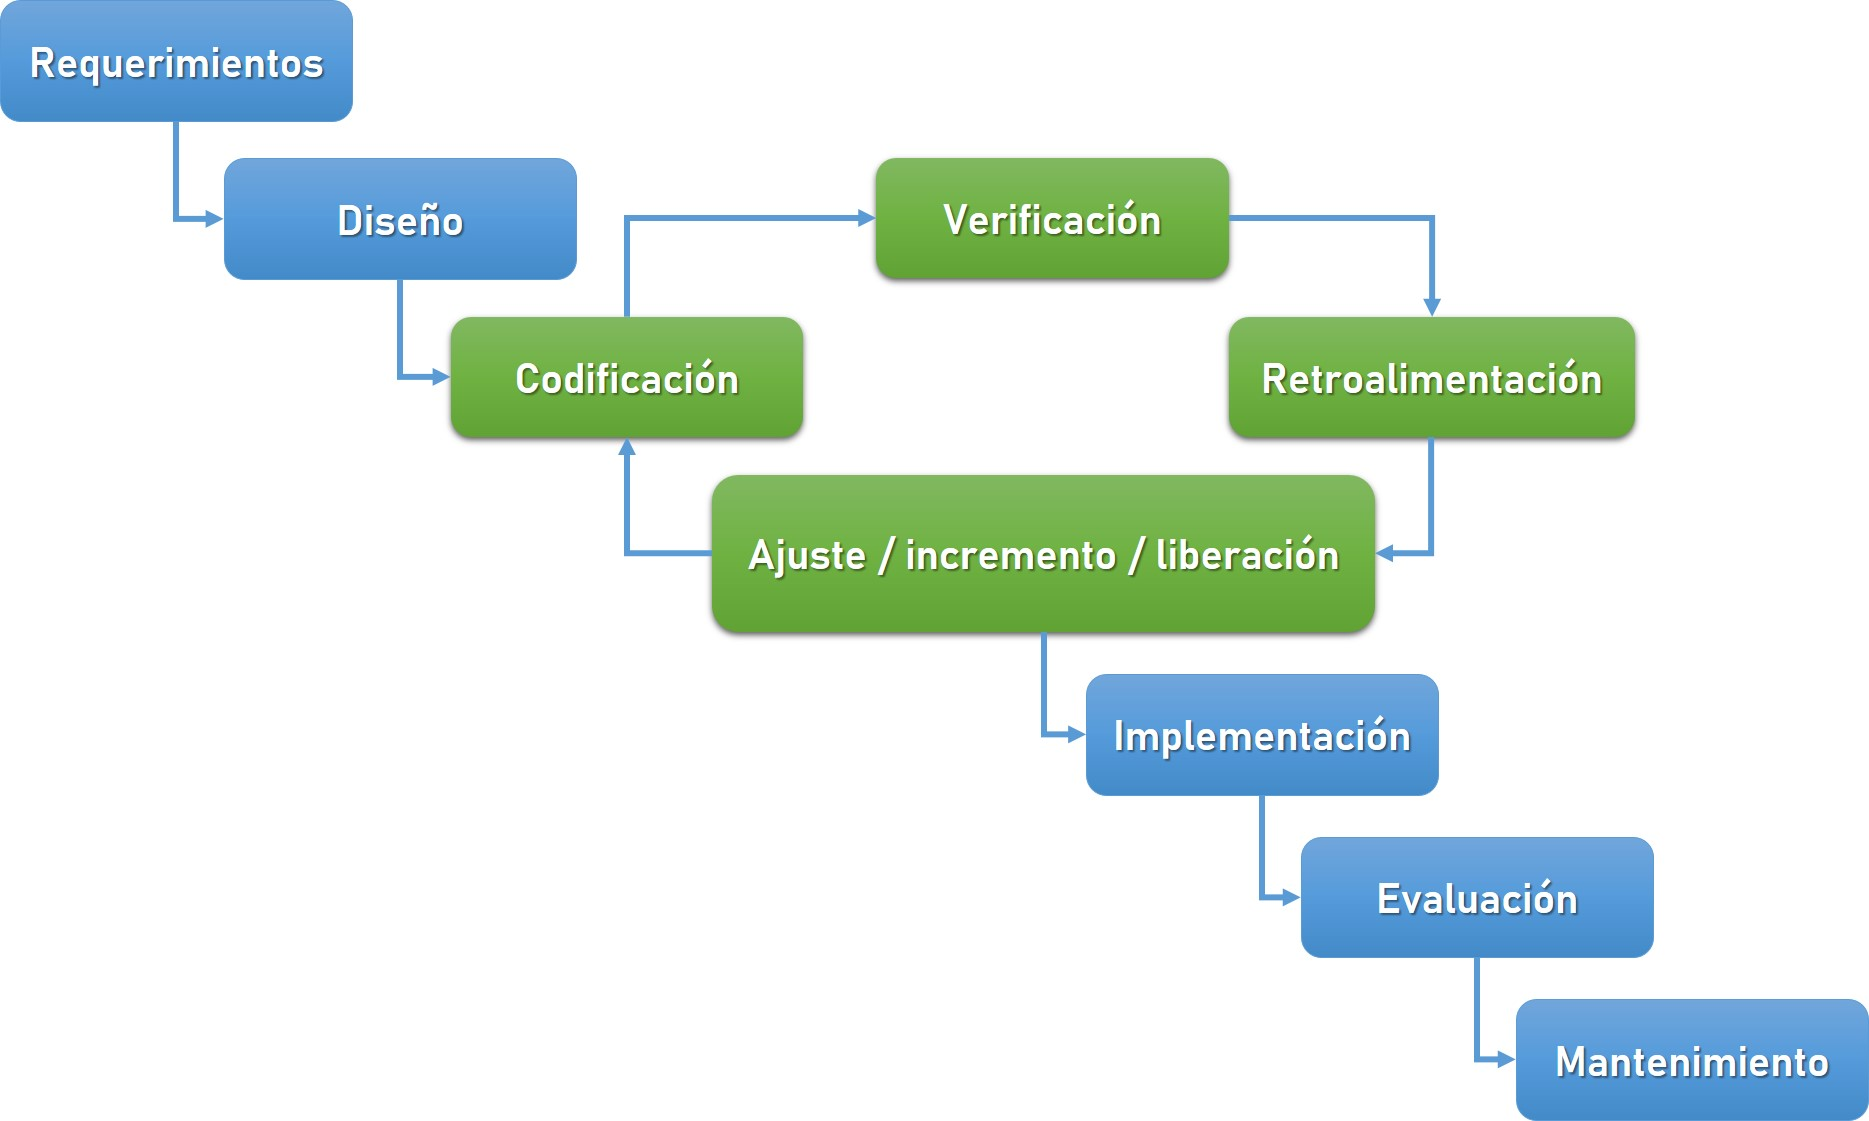
\includegraphics[width=12cm]{figures/ModeloDesarrolloSW.jpg}}
    \caption{Modelo de desarrollo del servicio web} %PIE DE LA IMAGEN
    \label{modeloDesarrolloSW}
\end{figure}

\section{An\'alisis de requerimientos}

Dado que el servicio web que se plantea implementar es parte del backend del RI-UPPue como un servicio especializado adicional, el usuario final n\'unca tendr\'a una interacci\'on con \'este, sino que el servicio trabajar\'a de manera trasparente proporcionando los resultados que le sean solicitados tal como una especie de gestor.\newline

Por lo anterior y en conjunto con la administradora del RI-UPPue se identificaron tanto las caracter\'isticas funcionales, como las de comportamiento considerados en la Tabla \ref{tablaRequerimientos}. \newline

\begin{table}[htbp]
    \begin{center}
    \caption{Tabla de requerimientos generales del servicio web}
    \begin{tabular}{| p{1.5cm}| p{8cm} |p{2cm} |}
    \hline
    \centering \textbf{No. } & \textbf{Descripci\'on} & \textbf{Prioridad} \\
    \hline \hline
    1 & Consulta de informaci\'on sem\'antica & Alta  \\ \hline
    2 & Capacidad de almacenamiento de ternas en RDF & Alta  \\ \hline
    3 & Exportaci\'on de datos en formatos no propietarios como JSON y RDF & Mediana  \\ \hline
    4 & Integraci\'on de datos provenientes de otros RIs & Mediana  \\ \hline
    \end{tabular}
    \label{tablaRequerimientos}
    \end{center}
\end{table}

\section{Dise\~{n}o}

Con el uso de un par de herramientas de modelado UML y basado en los requerimientos planteados en la etapa de an\'alisis se elaboraron modelos: de casos de uso, diagrama de clases y un dise\~{n}o de alto nivel del servicio web; los cuales de describe a continuaci\'on.

\subsection{Casos de uso}

En la Figura \ref{casoUso1} se muestra el diagrama de casos de uso que modela la funcionalidad general del RI-UPPue identificando los actores que interactuan con \'el y las actividades que realizan cada uno por su cuenta.\newline

\begin{figure}[!ht]
	\centering
	\fbox{
	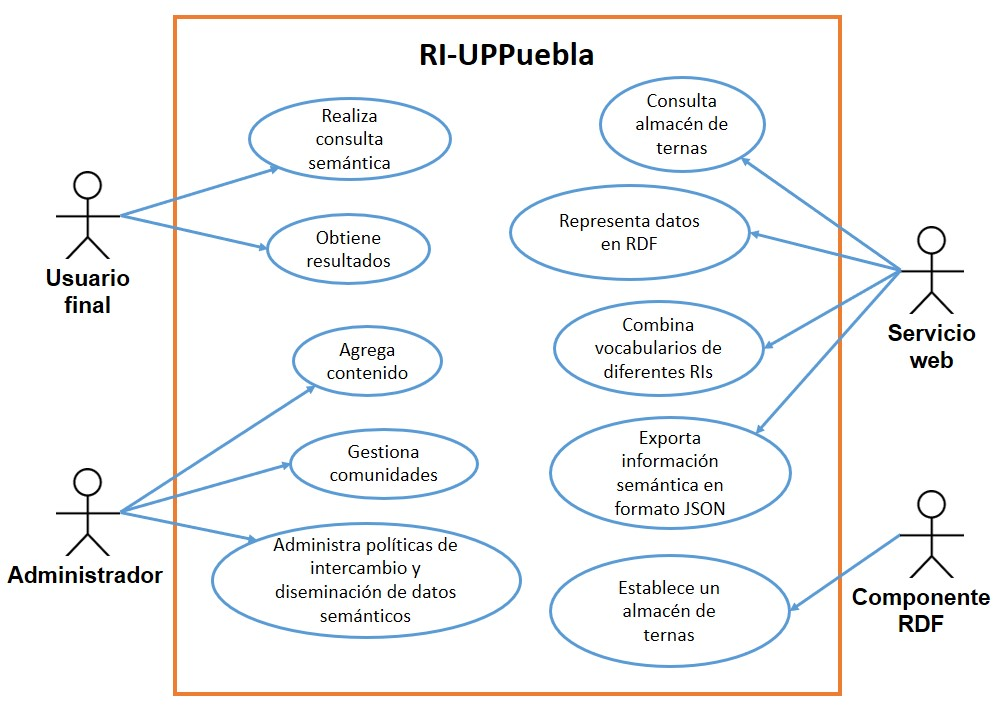
\includegraphics[width=12cm]{figures/CasoDeUso.jpg}} %NOMBRE DE LA FIGURA y TAMA\~{n}O
    \caption{Modelo de casos de uso} %PIE DE LA IMAGEN
    \label{casoUso1}
\end{figure}

\subsection{Diagrama de clases}

La Figura \ref{diagramaClases1} muestra el diagrama de clases del servicio web, donde a trav\'es de rect\'angulos en color verde se indican los nombres de las clases consideradas. En \cite{SOMIdiseno} se propone el siguiente dise\~{n}o anexando una descripci\'on detallada de atributos y m\'etodos definidos para cada clase.

\begin{figure}[!ht]
	\centering
	\fbox{
	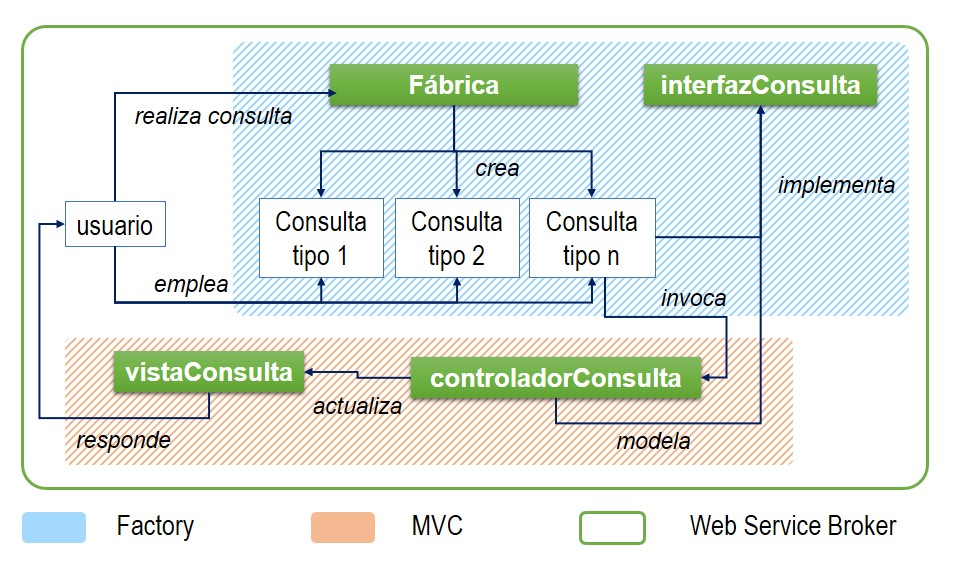
\includegraphics[width=12cm]{figures/Diagramadeclases1.jpg}} %NOMBRE DE LA FIGURA y TAMA\~{n}O
    \caption{Diagrama de clases. Fuente: \cite{SOMIdiseno}} %PIE DE LA IMAGEN
    \label{diagramaClases1}
\end{figure}

\subsection{Dise\~{n}o de alto nivel}

Las Figuras \ref{disenoAlto1} y \ref{disenoAlto2} muestran los dise\~{n}os elaborados para representar por un lado la manera en que se puede emplear el servicio web, y por otro lado, un modelo general del comportamiento del mismo, en el contexto general, donde en una primera instancia se operar\'a de manera local instalado en el servidor de RI-UPPue y posteriormente, se buscar\'a su instalaci\'on en diferentes RIs que compartan la misma plataforma tecnol\'ogica.

\begin{figure}[!ht]
	\centering
	\fbox{
	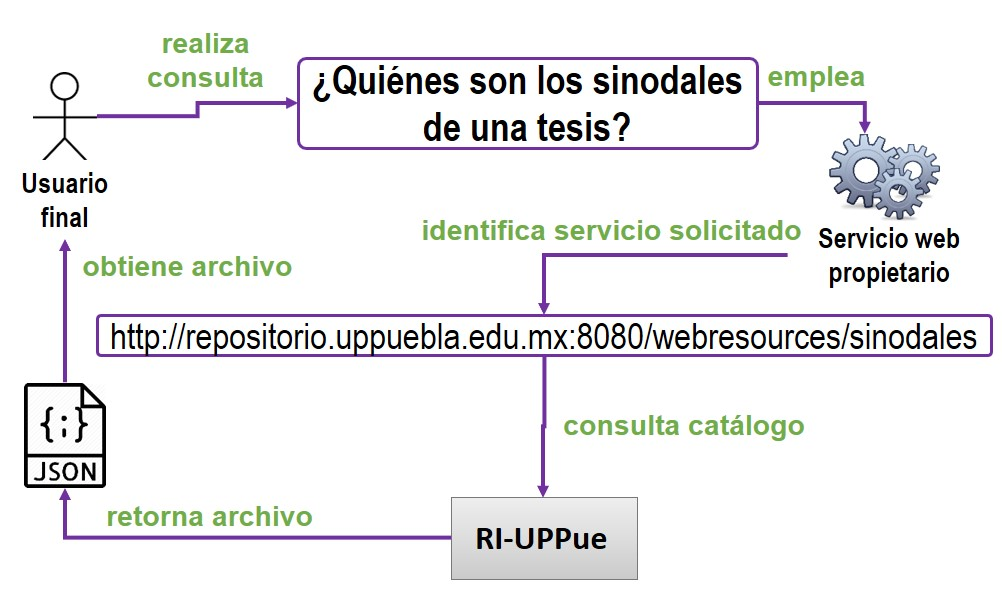
\includegraphics[width=12cm]{figures/DisenoAltoNivel1.jpg}} %NOMBRE DE LA FIGURA y TAMA\~{n}O
    \caption{Dise\~{n}o de consumo del servicio web. Fuente: \cite{SOMIdiseno}} %PIE DE LA IMAGEN
    \label{disenoAlto1}
\end{figure}

\begin{figure}[!ht]
	\centering
	\fbox{
	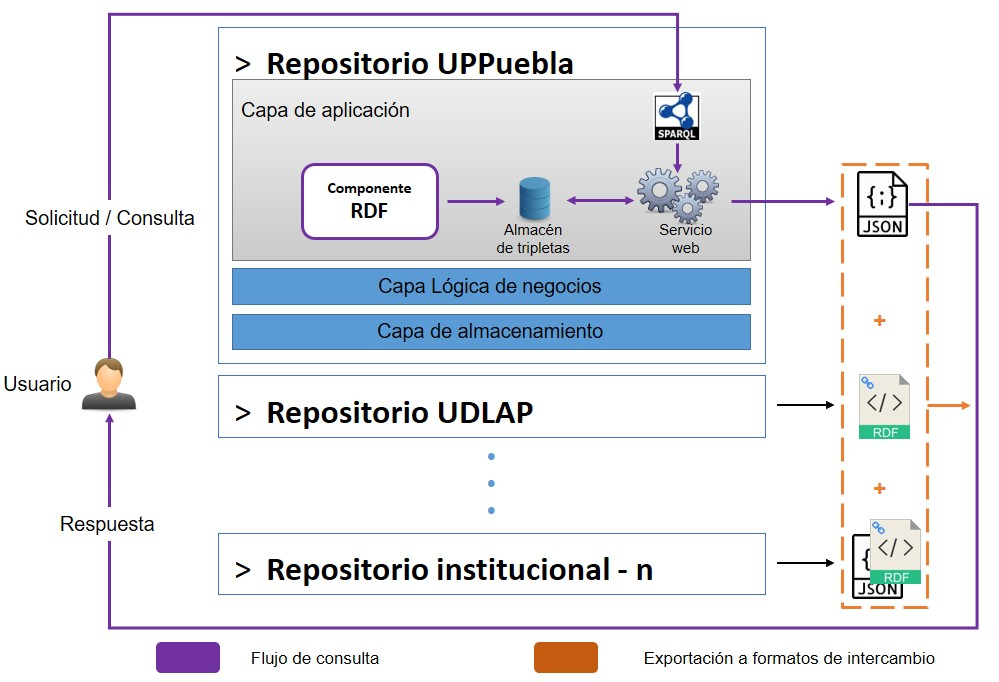
\includegraphics[width=12cm]{figures/DisenoAltoNivel2.jpg}} %NOMBRE DE LA FIGURA y TAMA\~{n}O
    \caption{Dise\~{n}o de alto nivel del servicio web. Fuente: \cite{SOMIdiseno}} %PIE DE LA IMAGEN
    \label{disenoAlto2}
\end{figure}

\section{Implementaci\'on}

Previo al desarrollo de alg\'un modulo y la implementaci\'on del mismo en el servidor donde se encuentra instalada la plataforma DSpace 6.2 es necesario realizar algunas actividades previas sin las cuales el servicio no podr\'ia operar.

\subsection{Pre-requisitos}

La Figura \ref{adicionalesDspace} muestra la arquitectura de la plataforma DSpace donde se observan los servicios adicionales que pueden ser habilitados para la plataforma DSpace en su versi\'on 6.2. La documentaci\'on de referencia de \cite{DSpaceRef} se indica que DSpace cuenta con un m\'odulo RDF, sin embargo, \'este no se encuentra habilitado en la instalaci\'on est\'andar del servidor.\newline

\begin{figure}[!ht]
	\centering
	\fbox{
	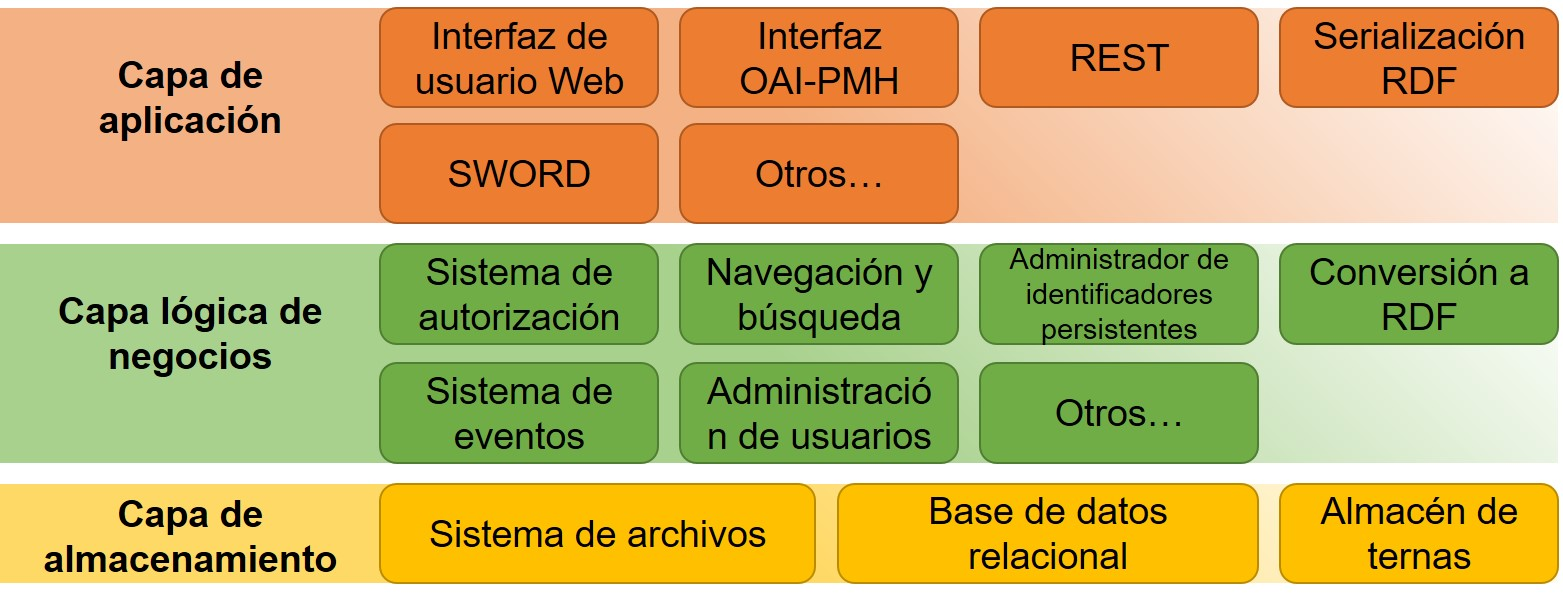
\includegraphics[width=12cm]{figures/ModulosAdicionalesDSpace62.jpg}} %NOMBRE DE LA FIGURA y TAMA\~{n}O
    \caption{M\'odulos adicionales de DSpace 6.2} %PIE DE LA IMAGEN
    \label{adicionalesDspace}
\end{figure}

La habilitaci\'on del m\'odulo de serializaci\'on RDF requiere de tres elementos de software: 1) un almac\'en de ternas, 2) un mecanismo de serializaci\'on y 3) un conversor a formato RDF. La instalaci\'on de estos elementos forman parte de las etapas del proceso t\'ecnico como muestra la Figura \ref{etapasMigracion}. Estas etapas se describen en las secciones siguientes.

\begin{figure}[!ht]
	\centering
	\fbox{
	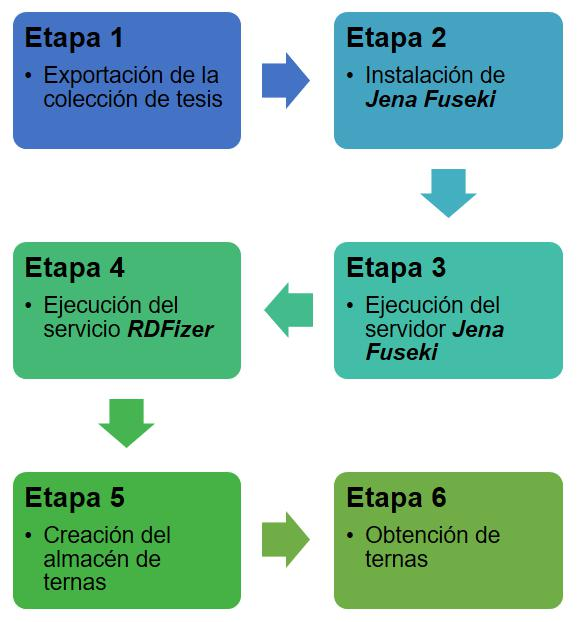
\includegraphics[width=10cm]{figures/etapasMigracion.jpg}} %NOMBRE DE LA FIGURA y TAMA\~{n}O
    \caption{Etapas del proceso de migraci\'on de metadatos del RI-UPPue a la web sem\'antica} %PIE DE LA IMAGEN
    \label{etapasMigracion}
\end{figure}

\subsubsection{Etapa 1. Exportaci\'on de la colecci\'on de tesis}

DSpace permite exportar cualquier colecci\'on, en este art\'iculo se reporta la de tesis del RI-UPPue. La Figura \ref{exportacion-csv} muestra interfaz para esta tarea, los metadatos se almacenan a un archivo de tipo CSV\footnote{Siglas del ingl\'es, Comma Separated Values, formato separado por comas}. El n\'umero 1 muestra el bot\'on para exportar y el 2 el archivo CSV con los metadatos exportados. La tarea se llev\'o a cabo al utilizar la versi\'on 75.0.3770.142 del navegador Chrome y la interfaz en JSP de DSpace.

\begin{figure}[!ht]
	\centering
	\fbox{
	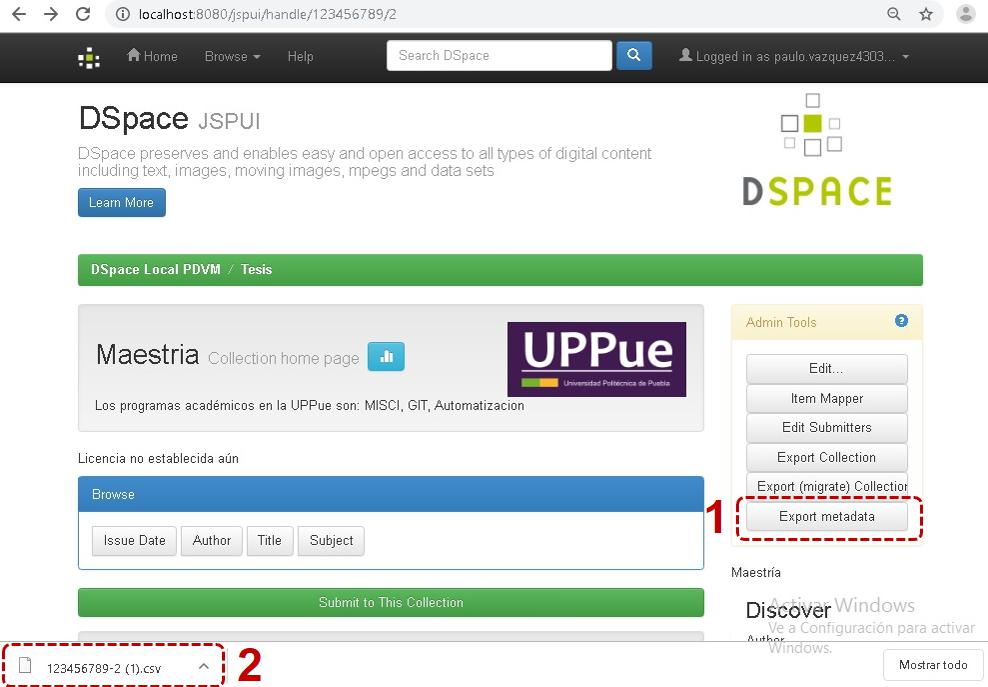
\includegraphics[width=12cm]{figures/exportarCSV.jpg}} 
    \caption{Exportaci\'on de la colecci\'on tesis a \textit{CSV}}
    \label{exportacion-csv}
\end{figure}

\subsubsection{Etapa 2. Instalaci\'on de Apache Jena Fuseki}

El almac\'en de ternas o servidor seleccionado fue Jena-Fuseki versi\'on 1.6.0, \'este provee tambi\'en de una interfaz web para realizar consultas en lenguaje SPARQL\footnote{SPARQL es un lenguaje de consultas para datos en RDF}. \newline

Fuseki se integra con TDB\footnote{Componente de Jena Fuseki para el almacenamiento y consulta de datos en RDF} para proporcionar una capa de almacenamiento persistente transaccional y robusta, permite consultas de texto y espaciales en Jena Fuseki\cite{JenaFuseki}. La p\'agina oficial de Apache Jena Fuseki\footnote{Disponible en https://jena.apache.org/download/index.cgi} provee diversas opciones para la descarga dependiendo del sistema operativo: Linux (.tar.gz) o Windows(.zip). \newline

\begin{figure}[!ht]
	\centering
	\fbox{
	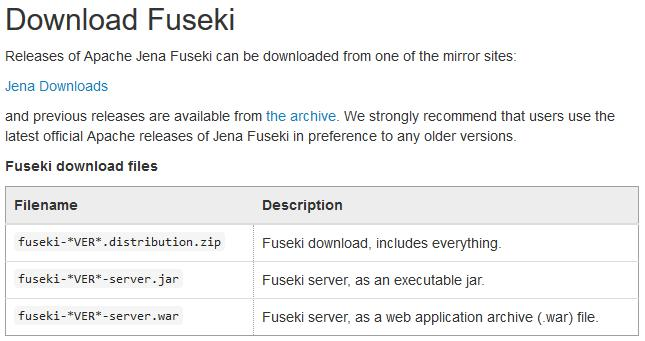
\includegraphics[width=12cm]{figures/opcionesDescargaFuseki.jpg}} 
    \caption{Opciones de descarga de Jena Fuseki}
\label{opcionesDescargaFuseki}
\end{figure}

Para terminar la instalaci\'on, los archivos se descomprimen, se guardan en una carpeta que se renombra como \textit{Fuseki} para poder ejecutar el servidor.\newline

\begin{figure}[!ht]
	\centering
	\fbox{
	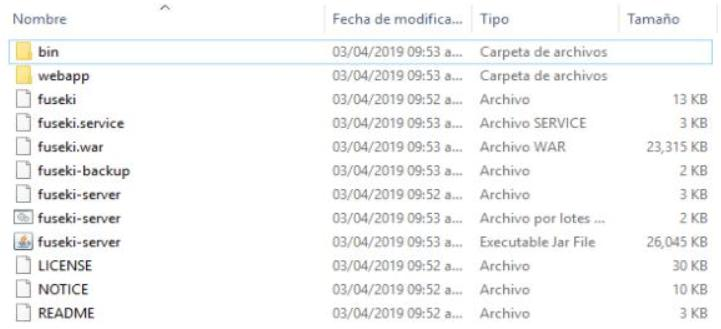
\includegraphics[width=12cm]{figures/contenidoCarpetaJena.jpg}} 
    \caption{Contenido de la carpeta del servidor \textit{Jena Fuseki}}
    \label{opcionesDescargaFuseki}
\end{figure}

\subsubsection{Etapa 3. Ejecuci\'on del servidor Jena Fuseki}

Jena Fuseki se ejecuta como servicio de sistema operativo, como aplicaci\'on web Java (WAR) o como servidor independiente. El componente Apache Shiro se utiliza para implementar caracter\'isticas de seguridad, tiene una interfaz de usuario para el monitoreo y la administraci\'on del servidor. Jena Fuseki se inicializa ejecutando el archivo \textit{fuseki-server.bat}, (\textit{.jar} en Linux) como muestra la Figura \ref{ejecucionFuseki}.\newline

\begin{figure}[!ht]
	\centering
	\fbox{
	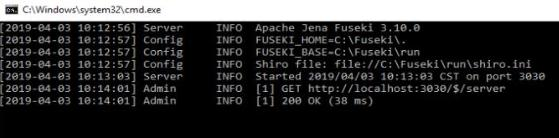
\includegraphics[width=12cm]{figures/ejecucionFuseki.jpg}} 
    \caption{Ejecuci\'on del servidor Jena Fuseki en terminal de Windows}
    \label{ejecucionFuseki}
\end{figure}

\subsubsection{Etapa 4. Ejecuci\'on del servicio RDFizer}

Un componente RDFizer\cite{RDFizer} o \textit{spongers}, transforma datos de DSpace en una o m\'as de las serializaciones al modelo de datos RDF. La Figura \ref{etl-diagrama} representa esta transformaci\'on. Los RDFizers implementan  las tareas b\'asicas siguientes: extraer, transformar y cargar, en ingl\'es, \emph{extract}, \emph{transform} y \emph{load} (ETL), mismas que se describen como sigue: 

\begin{itemize}
    \item \textit{Extraer}. Los datos se obtienen de una base de datos o se recopilan de fuentes m\'ultiples y diferentes
    
    \item \textit{Transformar}. Los datos obtenidos se transforman en los requeridos mediante formularios; la transformaci\'on utiliza reglas o tablas de b\'usqueda o combina los datos con otros.
    
    \item \textit{Cargar}. Los datos se escriben en la fuente o base de datos destino. 
\end{itemize}

\begin{figure}[!ht]
	\centering
	\fbox{
	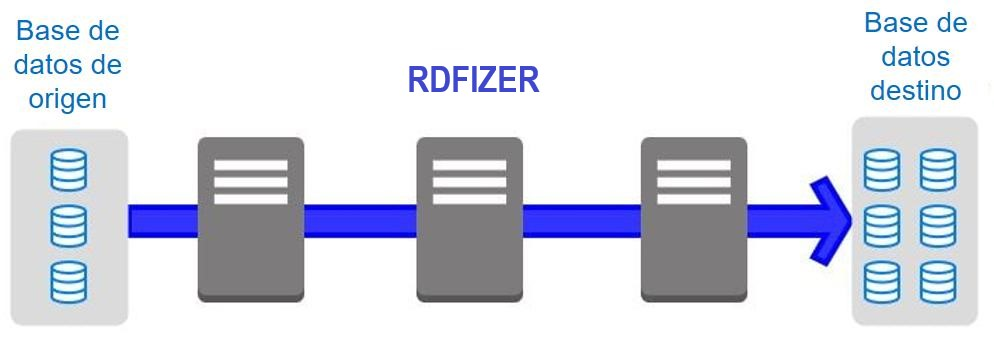
\includegraphics[width=12cm]{figures/etl.jpg}} 
    \caption{Extracci\'on, transformaci\'on y carga}
    \label{etl-diagrama}
\end{figure}

Los RDFizers soportan la migraci\'on de los metadatos a formatos de intercambio como XML, RDF, JSON. \newline

\subsubsection{Etapa 5. Creaci\'on del almac\'en de ternas}

Una vez que los metadatos del repositorio se han procesado por los RDFizes o ETLs, los archivos con datos en RDF se almacenan en la ubicaci\'on indicada en el archivo de configuraci\'on de la plataforma DSpace \textit{fuseki-assembler-ttl}, forman as\'i el almac\'en de ternas o servicio persistente.

\subsubsection{Etapa 6. Obtenci\'on de ternas}

Los metadatos en RDF para cada tesis se acceden empleando una direcci\'on de internet o URL\footnote{Localizador Uniforme de recursos, en ingl\'es \textit{Uniform Resource Locator}} como muestra la Figura \ref{accesoRdf}.\newline

\begin{figure}[!ht]
	\centering
	\fbox{
	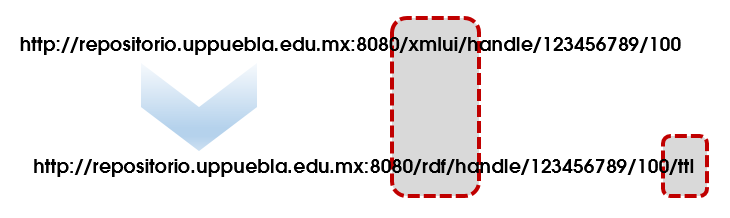
\includegraphics[width=12cm]{figures/xmluiRdf.png}} 
    \caption{Acceso a metadatos de tesis en RDF}
    \label{accesoRdf}
\end{figure}

La Figura \ref{resultadoRdf} muestra algunos metadatos de una tesis en RDF. Note que el archivo RDF contiene los metadatos capturados en la plataforma DSpace cuando se agrega un documento a la colecci\'on.

\begin{figure}[!ht]
	\centering
	\fbox{
	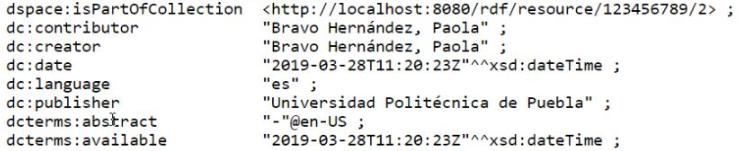
\includegraphics[width=12cm]{figures/extractoMetadatosRDF.jpg}} 
    \caption{Metadatos de RDF para una tesis del almac\'en de ternas}
    \label{resultadoRdf}
\end{figure}

\subsection{Servicio especializado en lenguaje Python 3.6}

El lenguaje de programaci\'on Python en su versi\'on 3.6 permite la extracci\'on de \'items almacenados en el almac\'en de ternas a trav\'es de la librer\'ia RDFLib \cite{RDFlib} versi\'on 4.2.2 y poder realizar actualizaciones en la ontolog\'ia Onto4-RI-UPPue a trav\'es de la librer\'ia OWLReady2 \cite{OWLReady2} versi\'on 0.19. La Figura \ref{arquitecturaServicio} muestra la arquitectura propuesta para el servicio web y cada uno de los componentes que lo componen.

\begin{figure}[!ht]
	\centering
	\fbox{
	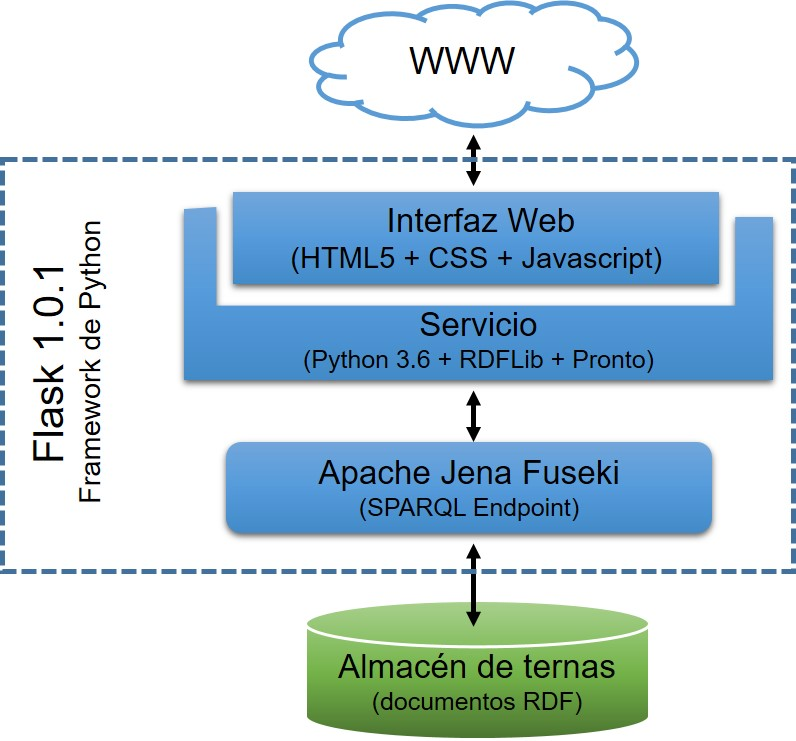
\includegraphics[width=10cm]{figures/ArquitecturaSW.jpg}} 
    \caption{Arquitectura del servicio web}
    \label{arquitecturaServicio}
\end{figure}

La Figura \ref{tecnologiasServicio} muestra un diagrama del tipo de tecnolog\'ias empleadas para el desarrollo del servicio web desde el punto de vista del \emph{Front end}\footnote{Parte gr\'afica del servicio web} y del \emph{Back end}\footnote{Parte l\'ogica del servicio web}.

\begin{figure}[!ht]
	\centering
	\fbox{
	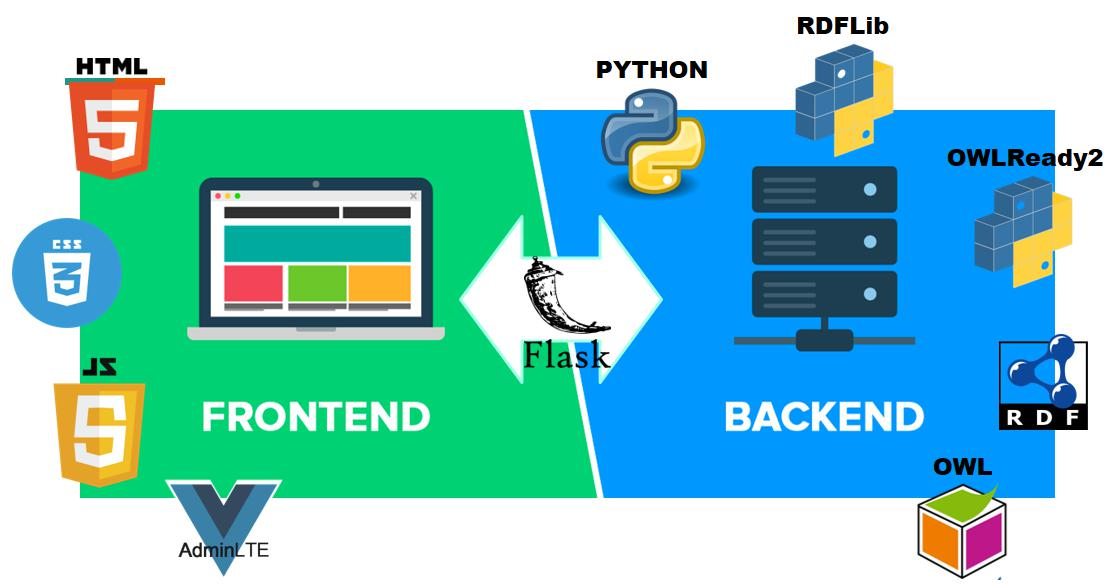
\includegraphics[width=12cm]{figures/tecnologiasServicoWeb.jpg}} 
    \caption{Tecnolog\'ias empleadas en el servicio web}
    \label{tecnologiasServicio}
\end{figure}

\subsubsection{Librer\'ia RDFLib}

La librer\'ia RDFLib \footnote{Disponible en: \textit{https://pypi.org/project/rdflib/}} es una biblioteca de Python para trabajar con RDF. La biblioteca contiene analizadores y serializadores para RDF / XML, N3, NTriples, Turtle, TriX, RDFa y Microdata. La biblioteca presenta una interfaz \textit{Graph} que puede ser respaldada por cualquiera de varias implementaciones de \textit{Store}. El n\'ucleo rdflib incluye implementaciones de tienda para almacenamiento en memoria, almacenamiento persistente en la parte superior de Berkeley DB y un contenedor para puntos finales SPARQL remotos, tambi\'en se incluye un motor SPARQL 1.1.\newline

La instalaci\'on de \'esta librer\'ia se realiza a trav\'es del servicio \textit{pip}\footnote{Repositorio de software para el lenguaje Python, en ingl\'es \textit{Python Index Package} } de Python, utilizando el comando \textit{pip install rdflib}, como lo indica la documentaci\'on oficial de la librer\'ia.\newline

\subsubsection{Librer\'ia OWLReady2}

La librer\'ia OWLReady2 \footnote{Disponible en \emph{https://pypi.org/project/Owlready2/}} Un paquete para la programaci\'on orientada a las ontolog\'ias en Python; carga de ontolog\'ias OWL 2.0 como objetos Python, modificaci\'on, actualizaci\'on y de razonadores como HermiT, adem\'as incluye un quadstore RDF optimizado.

La librer\'ia OWLReady2 permite realizar las siguientes actividades:

\begin{itemize}
    \item Importe ontolog\'ias OWL 2.0 en NTriples, RDF / XML o formato OWL / XML.
    \item Exportar ontolog\'ias OWL 2.0 a NTriples o RDF / XML
    \item Manipular clases, instancias y propiedades de ontolog\'ia de forma transparente, como si fueran objetos normales de Python
    \item Agregar m\'etodos de Python a las clases de ontolog\'ia
    \item Realizar la clasificaci\'on autom\'atica de clases e instancias, utilizando el razonador HermiT o Pellet (incluido)
    \item Cargar DBpedia o UMLS (para la terminolog\'ia m\'edica, utilizando el subm\'odulo PyMedTermino2 integrado)
    \item Soporte para mas de un bill\'on de ternas RDF
    \item Compatible con el m\'odulo RDFlib Python, que se puede usar para realizar consultas SPARQL
    \item Se puede usar como un ORM (mapeador relacional de objetos) - como una base de datos gr\'afica / objeto, supera a Neo4J, MongoDB, SQLObject y SQLAlchemy en t\'erminos de rendimiento
\end{itemize}

\subsubsection{Librer\'ia xml.etree.ElementTree}

La librer\'ia \textit{xml.etree.ElementTree}\footnote{Disponible en \textit{https://pypi.org/project/elementtree/}} permite parsear cualquier documento en formato XML por lo que, en el caso de prueba, la ontolog\'ia Onto4RI-UPPue que est\'a en formato OWL, puede ser editada mediante un objeto de tipo xml.etree.ElementTree cuyos m\'etodos pueden parsear y recorrer la ontolog\'ia mediante una estructura de \'arbol.\newline

Cuenta con diversos m\'etodos para parsear, acceder a elementos espec\'ificos de un documento, insertar, modificar y eliminar nodos en un XML.

\subsubsection{Framework Flask}

Para el desarrollo del servicio web se emplear\'a Flask versi\'on 1.1.1 \footnote{Disponible en \emph{https://pypi.org/project/Flask/}} el cual es un \emph{framework} \footnote{Un framework, entorno de trabajo​ o marco de trabajo​ es un conjunto estandarizado de conceptos, pr\'acticas y criterios para enfocar un tipo de problem\'atica particular que sirve como referencia, para enfrentar y resolver nuevos problemas de \'indole similar.} ligero para aplicaciones web. Est\'a dise\~{n}ado para desarrollar proyectos de manera r\'apida y f\'acil, con la capacidad de escalar a aplicaciones complejas. Es uno de los \emph{framework} de aplicaciones web de Python m\'as populares.\newline

Flask implementa de manera nativa el patr\'on de dise\~{n}o MVC\footnote{Modelo-Vista-Controlador, en ingl\'es \emph{Model-View-Controller}}, ampliamente usado en el desarrollo de proyectos de software. \newline

\subsubsection{Interfaz gr\'afica de usuario}

La \emph{GUI}\footnote{Interfaz gr\'afica de usuario} o \emph{Front end} del servicio integrar\'a tres tecnolog\'ias web: \emph{HTML5}\footnote{Lenguaje de modelado de hipertexto, en ingl\'es \emph{HiperText Markup Language}}, que es un lenguaje de marcado que sirve para modelar contenidos; \emph{Javascript}, que es un lenguaje de programaci\'on del lado del cliente que permite la manipulaci\'on de elementos HTML; y finalmente, \emph{CSS}\footnote{Hojas de estilo en cascada, en ingl\'es \emph{Cascading Style Sheets}}, que son hojas de estilo que permiten la definici\'on de reglas de dise\~{n}o, para la presentaci\'on del contenido.

Estas tecnolog\'ias son nativas a la web por lo que no se requiere de ning\'un tipo de instalaci\'on adicional, ya que la maquetaci\'on o ejecuci\'on de los modelos se realiza a trav\'es del uso de cualquier navegador web de \'ultima generaci\'on tales como: Chrome, Mozilla, Opera, Edge, Safari, etc.

Finalmente, en el desarrollo del \emph{Front end} se integrar\'a el uso del \emph{Dashboard}\footnote{Es un panel de control que conforma un tipo de interfaz gr\'afica de usuario} libre \emph{AdminLTE} en su versi\'on 2.4.15.

\section{Evaluaci\'on}

Las pruebas de usabilidad orientadas a la experiencia del usuario \footnote{Tambi\'en conocido como \emph{UX}, en ingl\'es \emph{User eXperience}} se basan en la observaci\'on y an\'alisis de un grupo de usuarios reales empleando el servicio web, con objeto de identificar los problemas de uso y poder solucionarlos.\newline

El servicio web ser\'a evaluado a trav\'es de una adaptaci\'on de la plantilla para hacer an\'alisis heur\'isticos de usabilidad\footnote{Disponible en \emph{https://www.torresburriel.com/weblog/2008/11/28/plantilla-para-hacer-analisis-heuristicos-de-usabilidad/}} propuesta por \cite{OnceHeuristicas}. La herramienta consta de un cuestionario que explora once heur\'isticas y en donde el evaluador (en este caso, un usuario) indica seg\'un una escala de Likert de cinco grados, su grado de satisfacci\'on. La Tabla \ref{tablaEscalasLikert} muestra las escalas con las que se evaluan cada una de las heur\'isticas.\newline

\begin{table}[htbp]
    \begin{center}
    \caption{Escalas Likert empleadas para evaluar el servicio web}
    \begin{tabular}{| p{1.5cm}| p{11cm} |}
    \hline
    \centering \textbf{Valor } & \textbf{Observaciones} \\
    \hline \hline
    1 & Se da la m\'inima expresi\'on del heur\'istico en las p\'aginas evaluadas \\ \hline
    2 & Se da una expresi\'on baja del heur\'istico en las p\'aginas evaluadas \\ \hline
    3 & Se da una expresi\'on media del heur\'istico en las p\'aginas evaluadas \\ \hline
    4 & Se da una expresi\'on alta del heur\'istico en las p\'aginas evaluadas \\ \hline
    5 & Se da la m\'axima expresi\'on del heur\'istico en las p\'aginas evaluadas \\ \hline
    \end{tabular}
    \label{tablaEscalasLikert}
    \end{center}
\end{table}

Las heur\'isticas evaluadas son las siguientes:

\begin{itemize}
    \item Generalidades
    \item Identidad e informaci\'on
    \item Lenguaje y redacci\'on
    \item Rotulado
    \item Estructura y navegaci\'on
    \item Estructura de la p\'agina
    \item B\'usqueda
    \item Elementos multimedia
    \item Ayuda
    \item Accesibilidad
    \item Control y retroalimentaci\'on
\end{itemize}

\begin{figure}[!ht]
	\centering
	\fbox{
	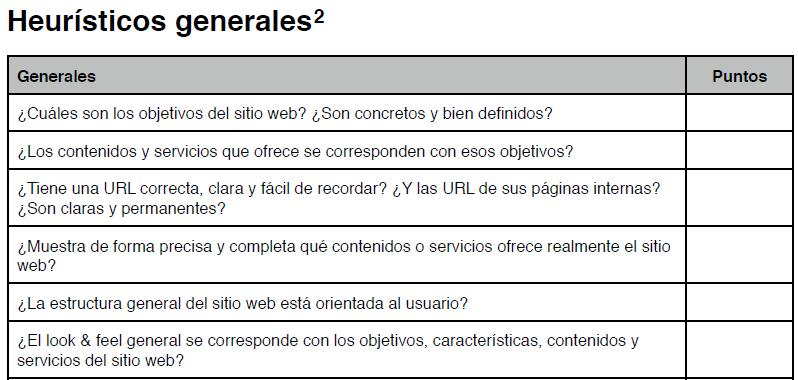
\includegraphics[width=12cm]{figures/extractoPlantilla.jpg}} 
    \caption{Extracto de la plantilla para hacer an\'alisis heur\'isticos de usabilidad}
    \label{extractoPlantilla}
\end{figure}

\section{Mantenimiento}

La fase final del desarrollo del servicio web consta de realizar las modificaciones o adecuaciones identificadas en la etapa de evaluaci\'on.
